\normaltrue \difficilefalse \tdifficilefalse
\correctionfalse

%\UPSTIidClasse{11} % 11 sup, 12 spé
%\newcommand{\UPSTIidClasse}{12}
% ATS 2019
\exer{Véhicule à trois roues Clever$\star$ \label{A3:05:80}}
\setcounter{numques}{0}
\UPSTIcompetence[2]{A3-05}
\index{Compétence A3-05}
\index{Véhicule à trois roues Clever}
\index{Caractériser un constituant de la chaîne de puissance.}
\index{Distributeur}
\index{Vérin}
\ifcorrection
\else
\textbf{Pas de corrigé pour cet exercice.}
\fi




On s'intéresse au véhicule à 3 roues Clever.

\ifprof
\else
%\begin{marginfigure}
%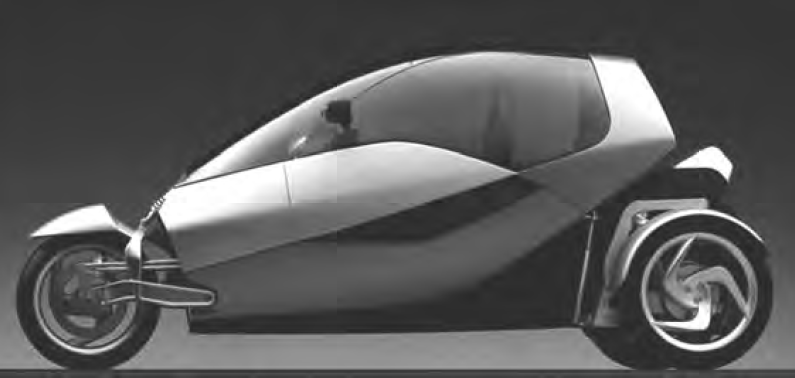
\includegraphics[width=.8\linewidth]{fig_80_01}
%%\textit{}
%\end{marginfigure}


 Le groupe motopropulseur est placé à l'arrière du véhicule. À l’avant, l’habitacle repose sur une roue de moto et pivote par rapport au bloc arrière autour d’une liaison pilotée angulairement par le biais de deux vérins hydrauliques. L'inclinaison est contrôlée par un ordinateur de bord en fonction de l'angle au volant et de la vitesse. 

\begin{center}
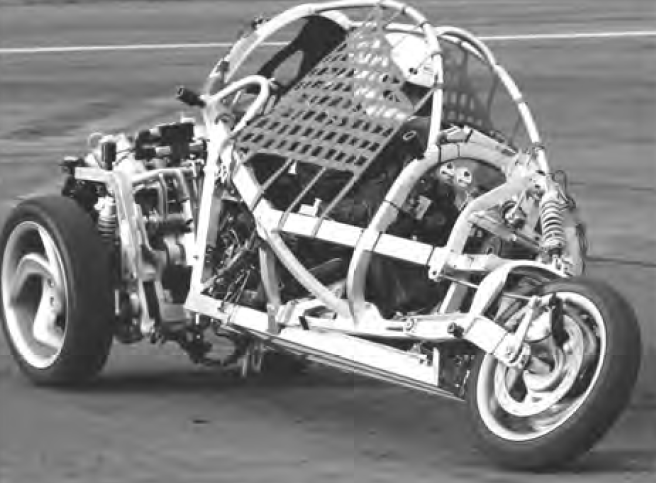
\includegraphics[width=.8\linewidth]{fig_80_02}
%\textit{}
\end{center}

%Le système d’inclinaison de l’habitacle est assuré par un système constitué :
%\begin{itemize}
%\item d’un calculateur qui détermine le mouvement et la position à donner à l’habitacle en fonction des conditions
%d’utilisation;
%\item d’un système hydro-mécanique de transmission de puissance et d’adaptation de mouvement;
%\item d’un système de contrôle de l’inclinaison de l’habitacle.
%\end{itemize}

La chaîne de transmission de puissance et d’adaptation de mouvement est composée :
\begin{itemize}
\item d’une pompe à engrenages actionnée par le moteur à gaz via un système de poulies/courroie;
\item d’un circuit hydraulique;
\item de 2 vérins hydrauliques simple effet;
\item d’un système mécanique d’adaptation de mouvement afin de transformer le mouvement de translation des tiges des vérins en rotation de l’habitacle.
\end{itemize}


\begin{center}
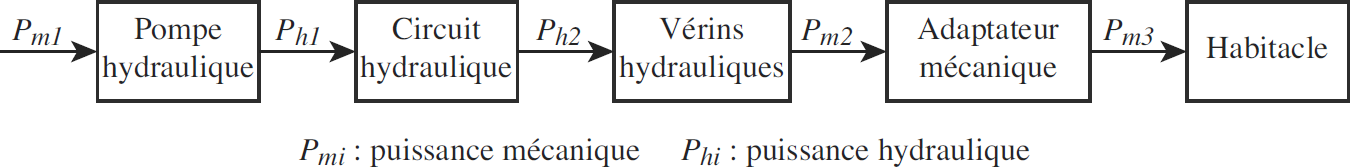
\includegraphics[width=\linewidth]{fig_80_03}
%\textit{}
\end{center}

\begin{center}
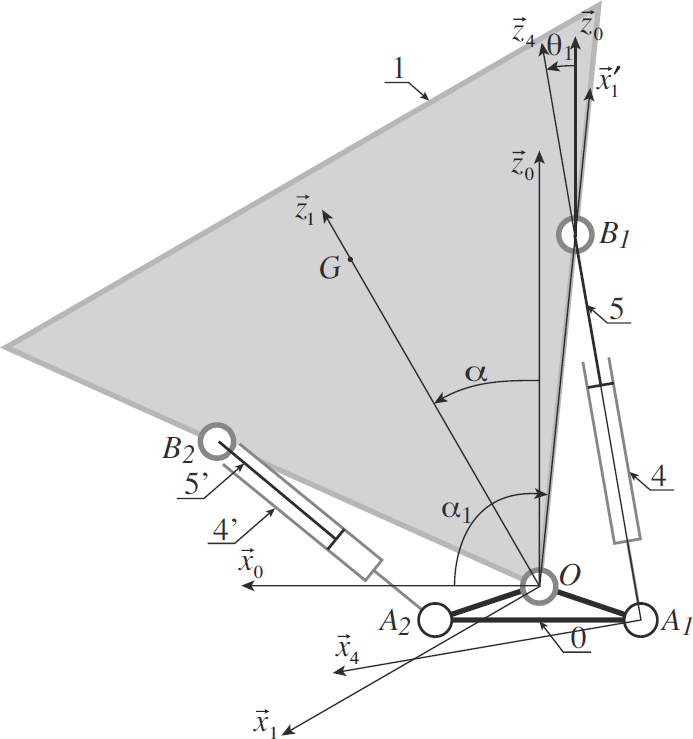
\includegraphics[width=.7\linewidth]{fig_80_04}
%\textit{}
\end{center}


Les deux vérins hydrauliques transforment la puissance hydraulique venant du servo-distributeur afin d’incliner l’habitacle. Ceux-ci sont disposées entre l’habitacle et le châssis du module arrière de propulsion. Le calculateur autorise ou non, l’alimentation en huile de l’un des vérins provoquant la sortie de tige, pendant que l’huile s'évacue de l’autre vérin. Ainsi l’habitacle s'incline du coté opposée au vérin alimenté. Lorsque l’habitacle est en position centrale, les tiges de vérins ont en position médiane.


Le circuit hydraulique est composé de 6 modules:
\begin{itemize}
\item une pompe à engrenages entraînée par le moteur à gaz;
\item un clapet anti-retour et une valve de décharge tarée pour s’enclencher à \SI{160}{bar} et se remettre en position fermée à \SI{100}{bar};
\item un accumulateur oléopneumatique de volume nominal \SI{1,4}{L};
\item un limiteur de pression;
\item un servo-distributeur à effet proportionnel 4/3 à centre fermé;
\item deux vérins simple effet, de diamètre \SI{32}{mm} pour chaque piston et de \SI{200}{mm} de course.
\end{itemize}

\fi

\question{Compléter le câblage du circuit hydraulique à partir du signe << * >>, ainsi que le schéma  du servo-distributeur.}

\ifprof
\begin{corrige}
\begin{center}
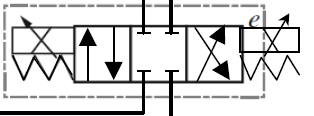
\includegraphics[width=.5\linewidth]{fig_80_cor_01}
%\textit{}
\end{center}
\end{corrige}
\else\begin{center}
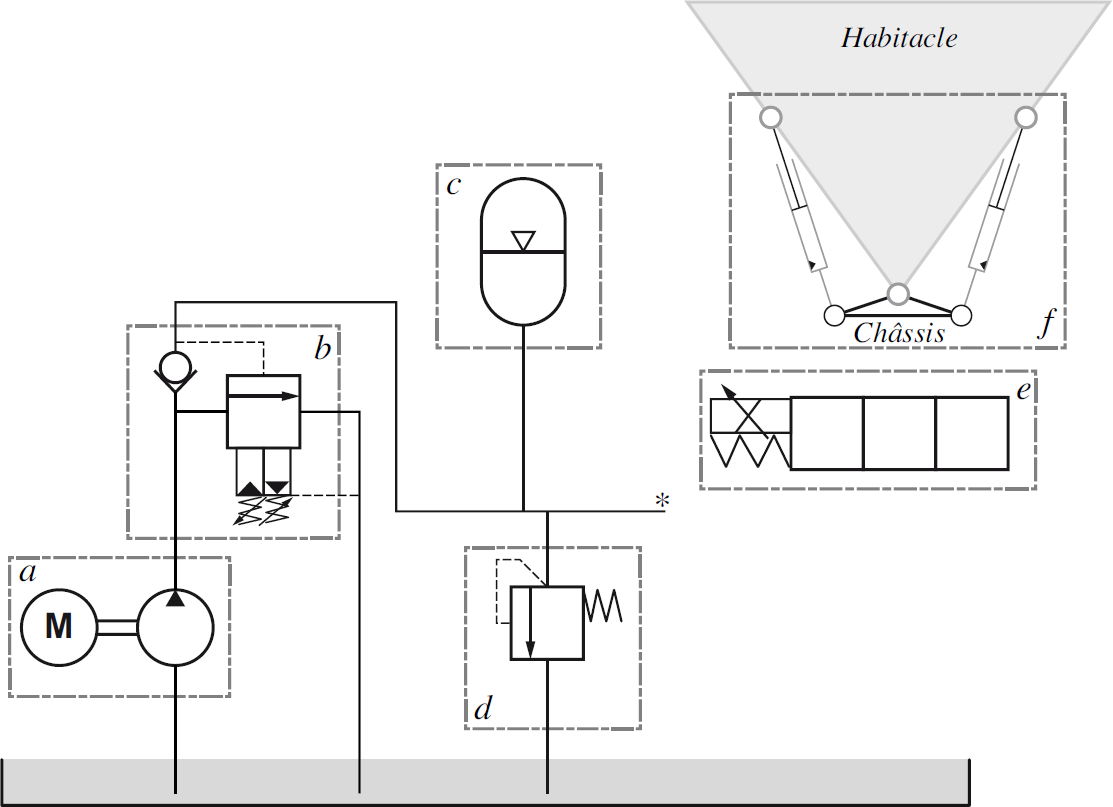
\includegraphics[width=\linewidth]{fig_80_05}
%\textit{}
\end{center}

\fi

Au démarrage du véhicule, la valve de décharge du module (b) est fermée. Le distributeur à effet proportionnel(e) est en position médiane, les vérins sont donc immobiles. La commande des vérins est initialement bloquée par une temporisation.

\question{En considérant les conditions initiales évoquées, expliquer, en commençant à l’instant de démarrage de la pompe, le comportement du circuit hydraulique en précisant clairement les différentes phases de fonctionnement. Quel est l’utilité de la temporisation ? On souhaite remplacer cette temporisation par un capteur. Préciser la grandeur qu’il devra mesurer. Donner un avantage et un inconvénient du remplacement de la temporisation par ce capteur.}
\ifprof
\begin{corrige}
Démarrage de la pompe et montée en pression du circuit avec remplissage de l’accumulateur (c).

À la fin de la temporisation le distributeur peut être commandé et ainsi alimenter les vérins.

Si la pression augmente trop, alors le limiteur de pression (d) renvoie une partie du fluide vers le
réservoir et si c’est insuffisant alors (b) permet une décharge du circuit (ouverture vers le réservoir
jusqu’à atteindre ne niveau bas réglé).

La temporisation permet d’attendre qu’un niveau de pression suffisant dans le circuit soit atteint.

Pour remplacer la temporisation on peut mesurer la pression dans le circuit ou plus simplement détecter
le niveau de pression satisfaisant pour le fonctionnement à l’aide d’un pressostat.

La solution utilisant un capteur de pression est plus sûre que la temporisation qui pourrait autoriser la
commande du distributeur alors que la pression dans le circuit est encore insuffisante.

(UPSTI). 
\end{corrige}
\else
\fi






\ifprof
\else
\begin{flushright}
\footnotesize{Corrigé  voir \ref{A3:05:80}.}
\end{flushright}%
\fi